\chapter{Time Will Tell: The role of mobile learning analytics in self-regulation} 


\vfill
Nowadays, smartphone users bla bla
\vspace{3em}

This chapter has been submitted as: 
Tabuenca, B., Kalz, M., \& Specht, M. (2015). (Submitted) Time Will Tell: The role of mobile learning analytics in self-regulation. \em Internet and Higher Education \em

\clearpage

\section{Introduction}

\subsection{Self-regulation with mobile technology}

\subsubsection{Psychology of notifications}

\subsubsection{Learning analytics}

\subsubsection{Seamless learning}

\section{Method}

\subsection{Participants}

\subsection{Materials}

\subsubsection{LearnTracker Backend}


\begin{figure}
     \centering
     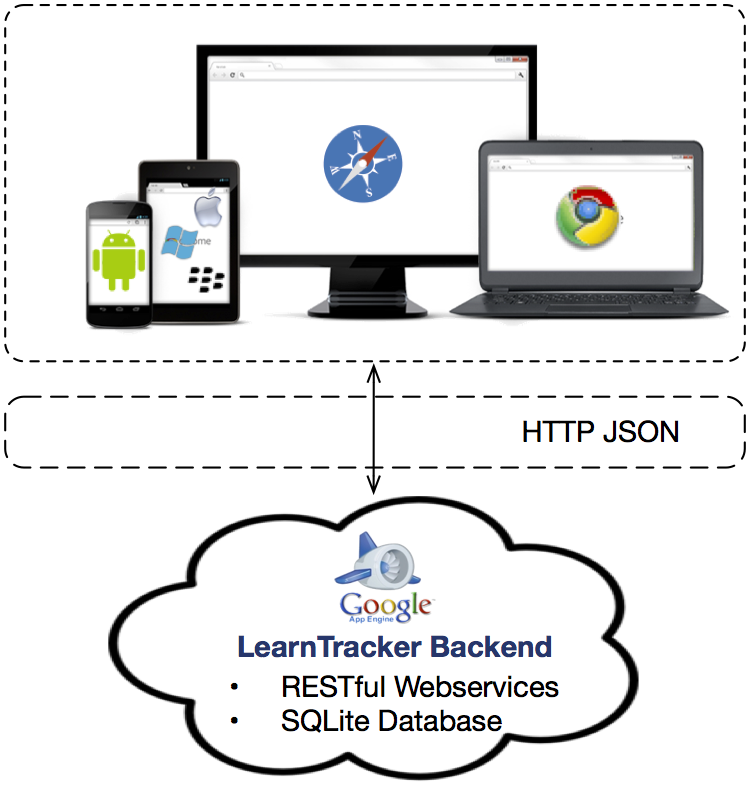
\includegraphics[width=0.7\linewidth]{img/studyload_fig1}
     \caption{LearnTracker's Backend outline}
     \label{fig:sload_1}
\end{figure}
\textbf{Database model}


\begin{figure}
     \centering
     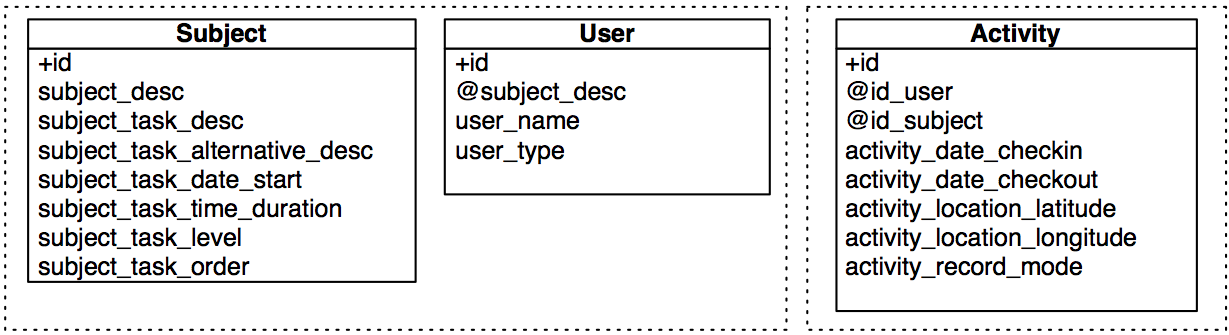
\includegraphics[width=0.7\linewidth]{img/studyload_fig2}
     \caption{LearnTracker's Backend database model}
     \label{fig:sload_2}
\end{figure}

\textbf{Webservices}


\subsubsection{Mobile clients}

\textbf{LearnTracker for Android}

\begin{center}
\begin{figure}[ht]
\centering
	\subfloat[Yardstick comprising activities scheduled in the GIS course]{
		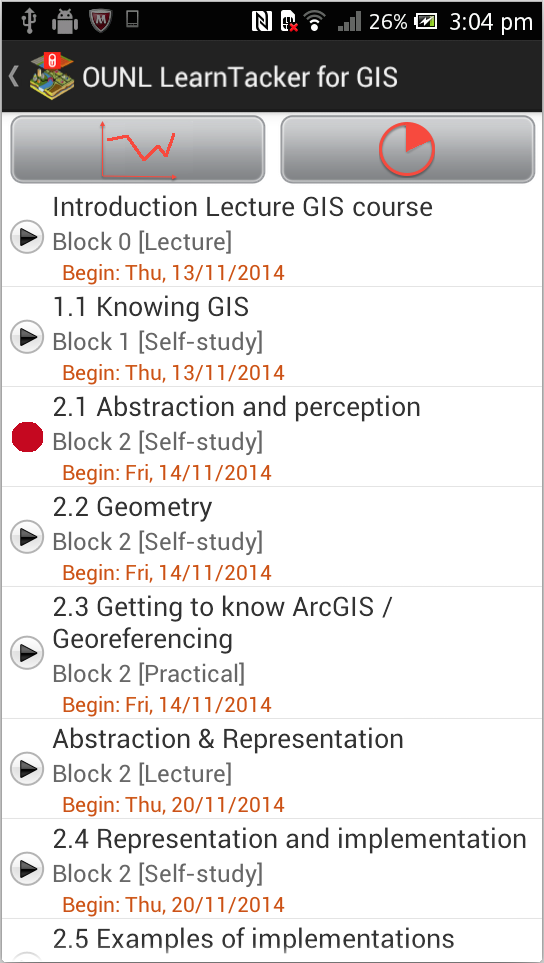
\includegraphics[width=0.3\linewidth]{img/studyload_fig3a}
		\label{fig:sload_3a}
	}
	\subfloat[Check-in: Tap to start learning activity ''2.1 Abstraction and perception'']{
		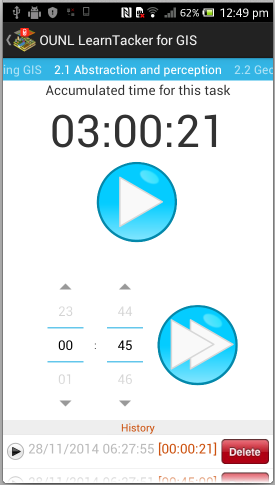
\includegraphics[width=0.3\linewidth]{img/studyload_fig3b}
		\label{fig:sload_3b}
	}	
	\subfloat[Check-out: Tap to stop learning activity  ''2.1 Abstraction and perception'']{
		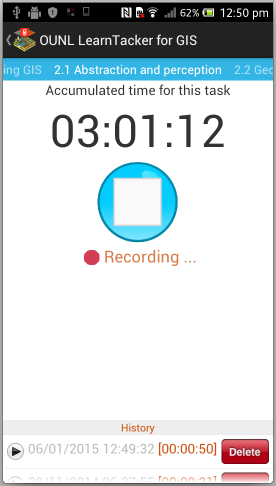
\includegraphics[width=0.3\linewidth]{img/studyload_fig3c}
		\label{fig:sload_3c}
	}	
      \caption{LearnTracker client for Android}
      \label{fig:sload_3}
\end{figure}
\end{center}

\begin{center}
\begin{figure}[ht]
\centering
	\subfloat[PieChart. Time devoted by a student on the activities in a course]{
		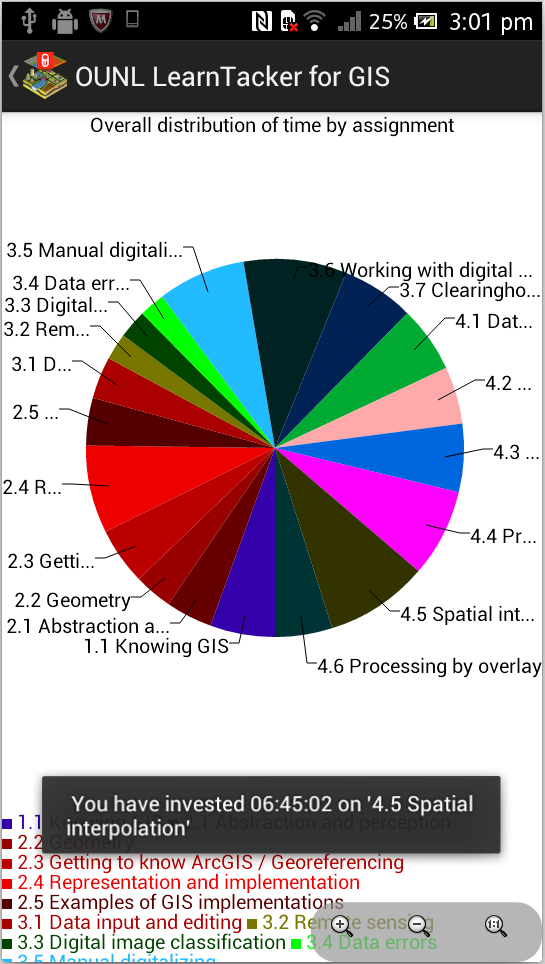
\includegraphics[width=0.3\linewidth]{img/studyload_fig4a}
		\label{fig:sload_4a}
	}
	\subfloat[Linechart. X-axis illus- trates activities in a course. Y-axis represents the number of hours devoted to study. My time (violet line) vs. My colleagues� time (black line)]{
		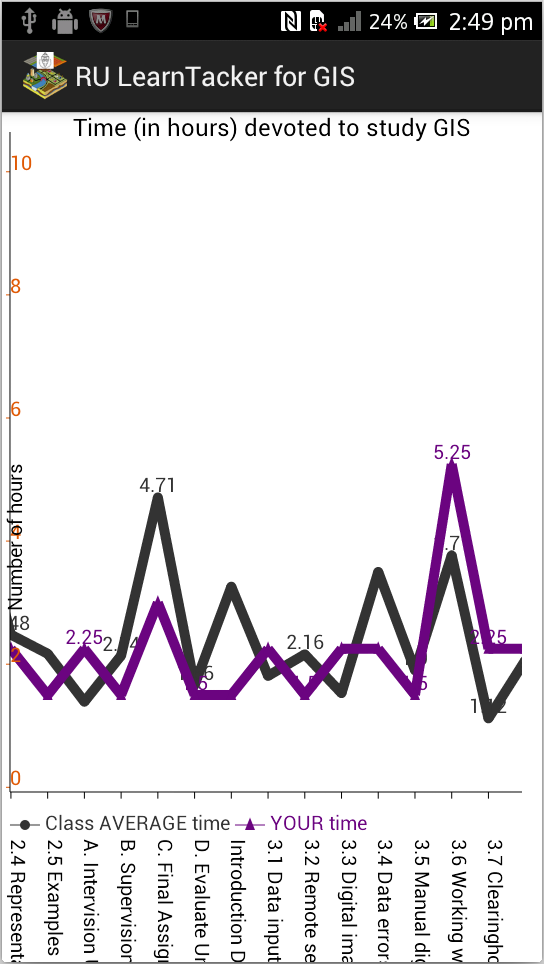
\includegraphics[width=0.3\linewidth]{img/studyload_fig4b}
		\label{fig:sload_4b}
	}	
	\subfloat[Linechart. X-axis illus- trates activities in a course. Y-axis represents number of hours devoted to study. My time (violet line) vs. My colleagues� time (red line) vs. My teacher� estimation (blue line)]{
		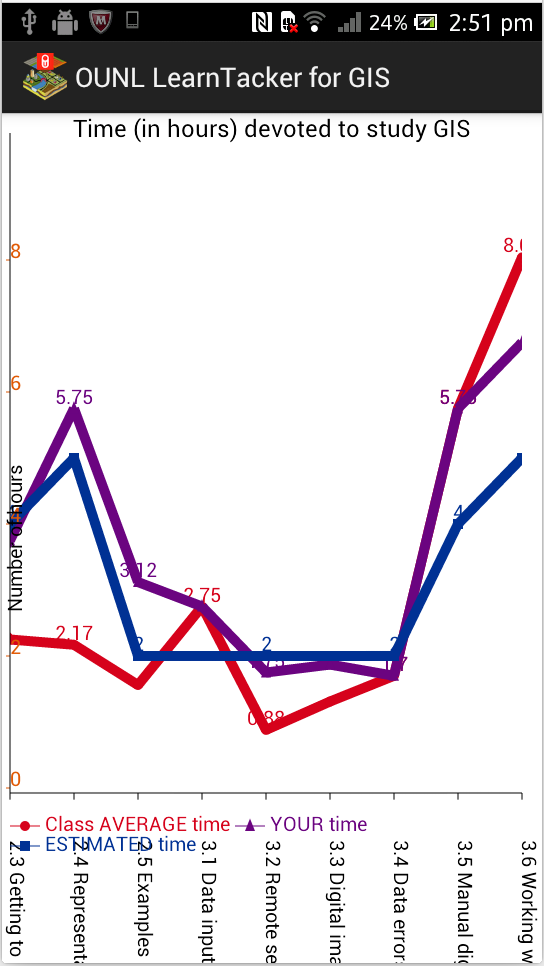
\includegraphics[width=0.3\linewidth]{img/studyload_fig4c}
		\label{fig:sload_4c}
	}	
      \caption{Learning analytics in LearnTracker}
      \label{fig:sload_4}
\end{figure}
\end{center}

\textbf{Multiplatform web interface}



\begin{center}
\begin{figure}[ht]
\centering
	\subfloat[Yardstick]{
		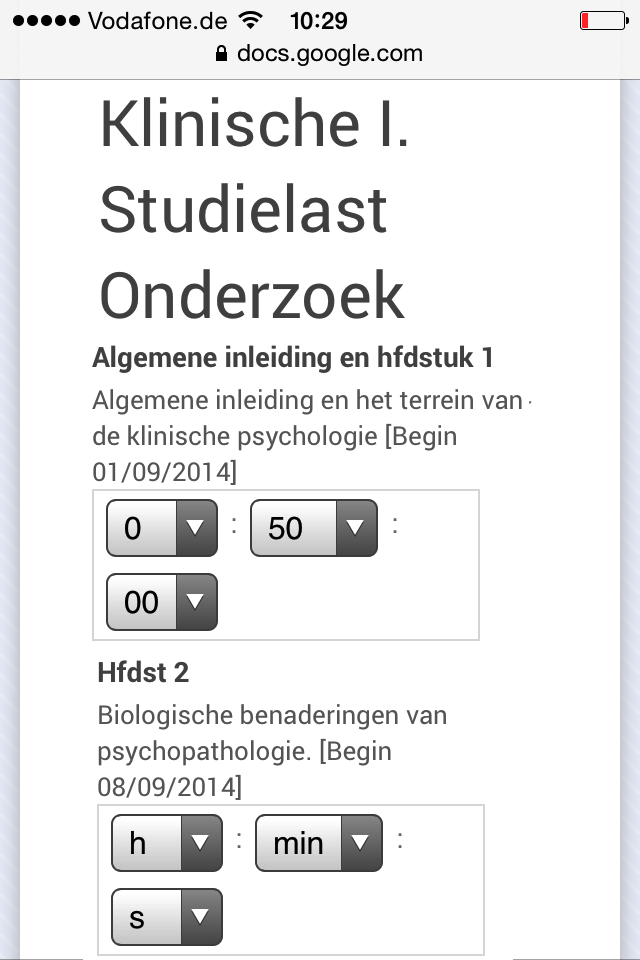
\includegraphics[width=0.3\linewidth]{img/studyload_fig5a}
		\label{fig:sload_5a}
	}
	\subfloat[Piechart. Time devoted to each learning activity]{
		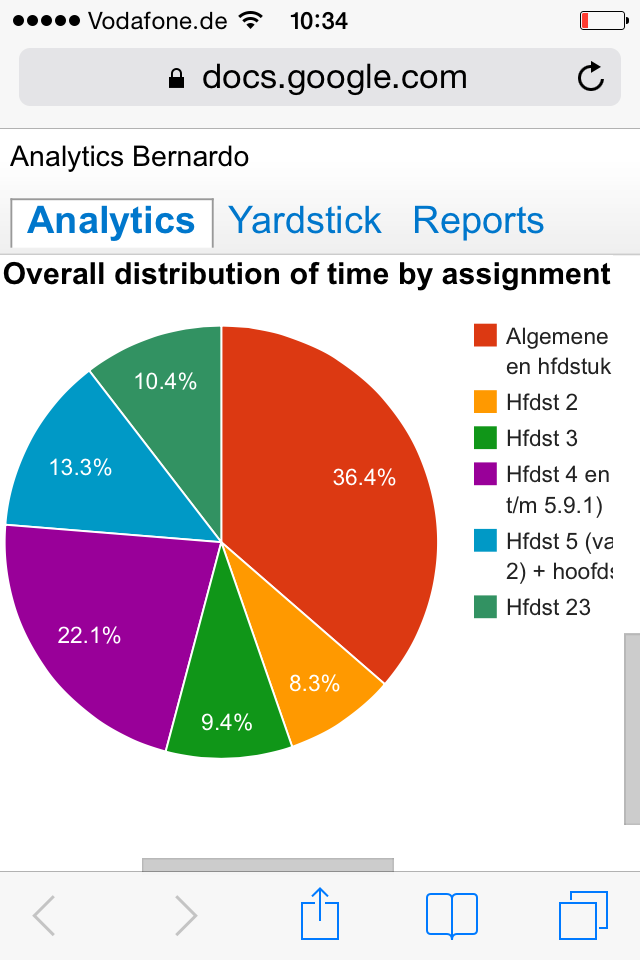
\includegraphics[width=0.3\linewidth]{img/studyload_fig5b}
		\label{fig:sload_5b}
	}	
	\subfloat[Barchart. My time VS time initially scheduled by the teacher]{
		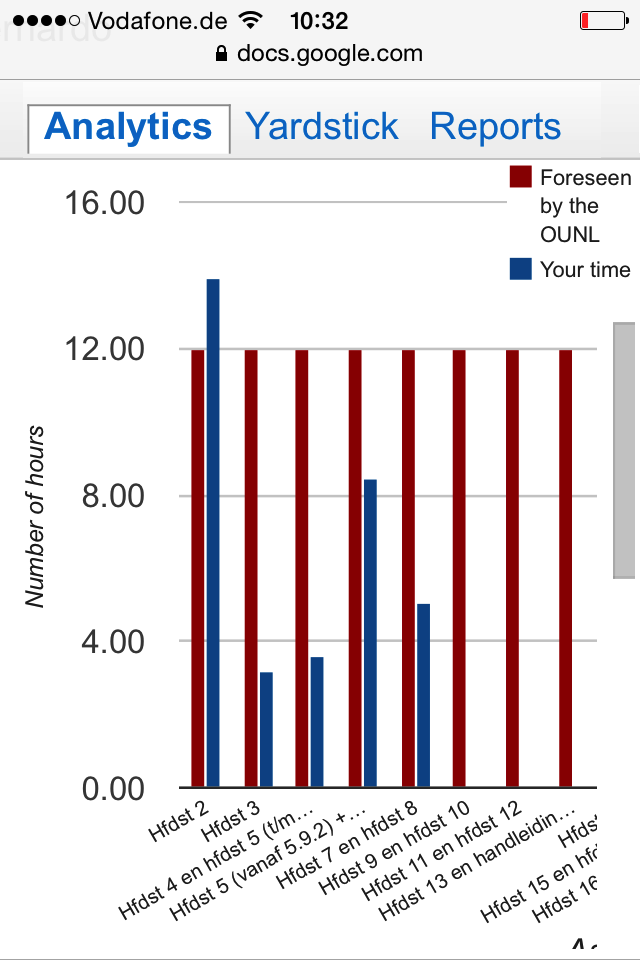
\includegraphics[width=0.3\linewidth]{img/studyload_fig5c}
		\label{fig:sload_5c}
	}	
      \caption{Multiplatform web interface}
      \label{fig:sload_5}
\end{figure}
\end{center}
\subsubsection{Notifications and SMS broadcasting tool}


\begin{center}
\begin{figure}[ht]
\centering
	\subfloat[SMS management tool]{
		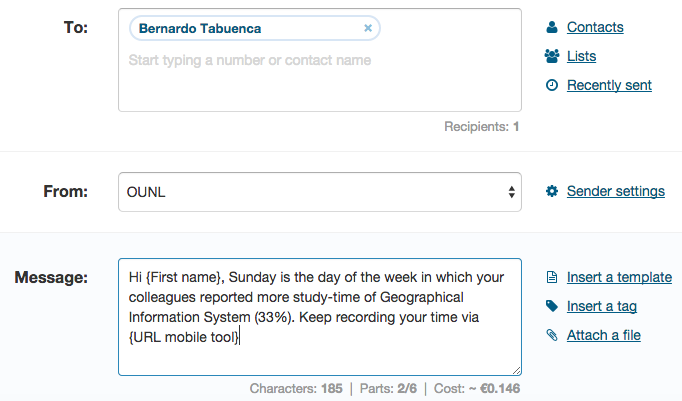
\includegraphics[width=0.3\linewidth]{img/studyload_fig6a}
		\label{fig:sload_6a}
	}
	\subfloat[SMSs generated out of the templates]{
		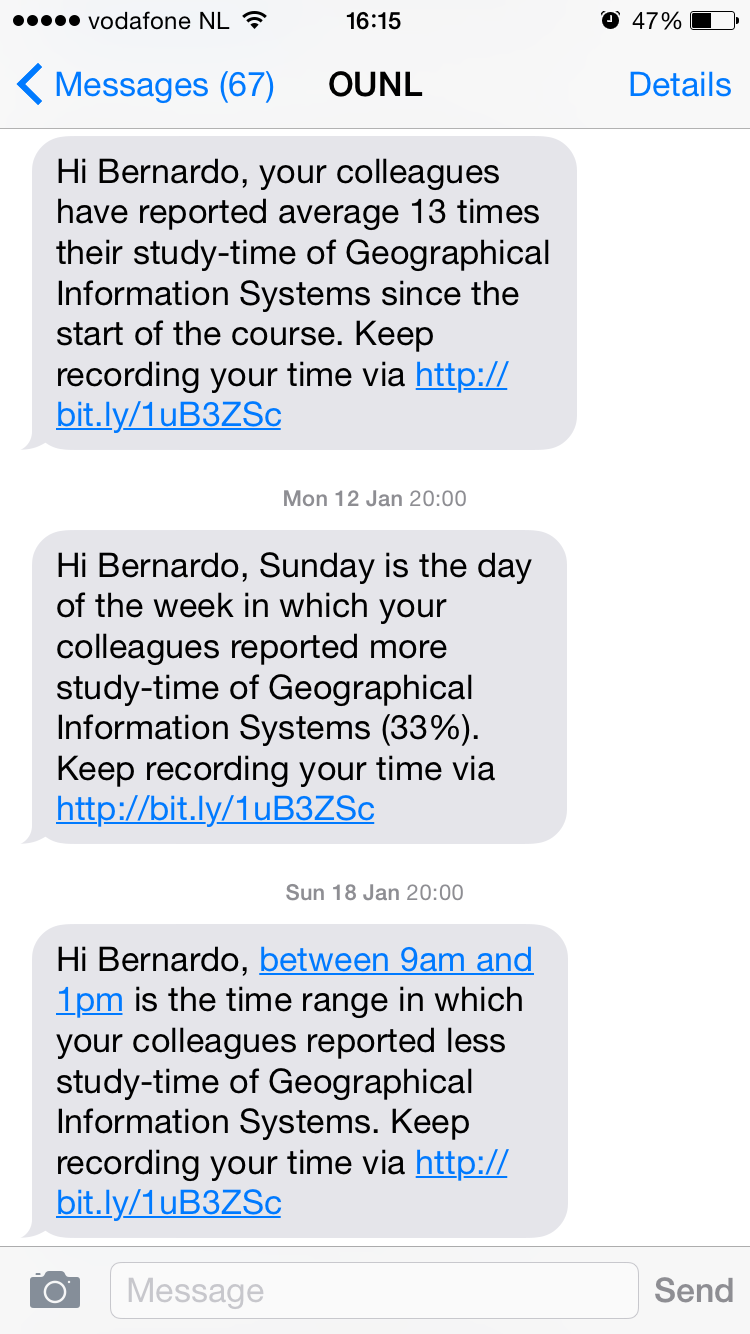
\includegraphics[width=0.3\linewidth]{img/studyload_fig6b}
		\label{fig:sload_6b}
	}		
      \caption{SMS broadcasting tool}
      \label{fig:sload_6}
\end{figure}
\end{center}
\subsection{Design of the experiment}


\begin{figure}
     \centering
     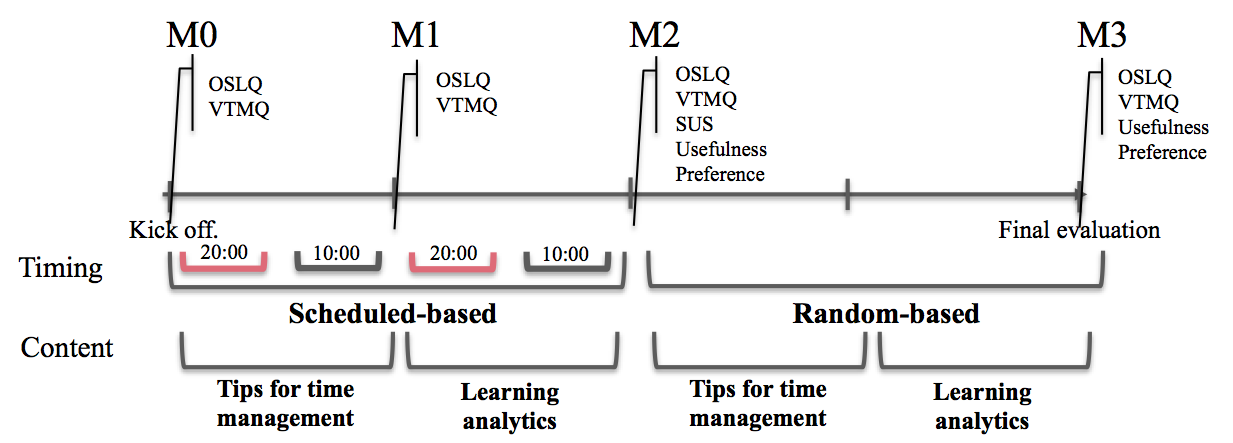
\includegraphics[width=0.7\linewidth]{img/studyload_fig7}
     \caption{Experimental design}
     \label{fig:sload_7}
\end{figure}
\subsection{Measure instruments}

\subsubsection{Self-regulation}

\subsubsection{Validity and reliability of time management}

\subsubsection{Time patterns}

\subsubsection{Complexity of the mobile tool}

\subsection{Procedure}

\subsection{Data analysis}

\section{Results}

\subsection{Impact of logging/monitoring time in self-regulation}



\begin{table}[h]
  \centering
  \small
  \caption{Internal consistency of OSLQ and VRTMQ (n=52). * Cronbach's alpha >=70}
  \label{tbl:studyload_table1}

\begin{tabular}{llcr}
\hline
\textbf{Scale} & \textbf{Subscale}                        & \textbf{Num. items} & \textbf{$\alpha$}                 \\
\hline
OSLQ           & Goal setting                             & 5                   & .83*                              \\
               & Environment structuring                  & 4                   & .78*                              \\
               & Time management                          & 3                   & .76*                              \\
               & Help seeking                             & 4                   & .69*                              \\
               & Self-evaluation                          & 4                   & .50                               \\
               & Task strategies                          & 4                   & .41                               \\
\textbf{}      & \multicolumn{1}{r}{\textbf{Total scale}} & \textbf{24}         & \textbf{.80*}                     \\
\hline
VTMQ           & Time planning                            & 16                  & .92*                              \\
               & Time attitudes                           & 7                   & .56                               \\
               & Time wasters                             & 4                   & .30                               \\
\textbf{}      & \multicolumn{1}{r}{\textbf{Total scale}} & \textbf{27}         & \multicolumn{1}{l}{\textbf{.89*}}\\ \hline
\end{tabular}
\end{table}


\begin{table}[h]
  \centering
  \small
  \caption{Means for the course C1. 5) Strongly disagree; 4) Disagree; 3) Neutral; 2) Agree; 1) Strongly agree; (*Friedman�s ANOVA significance: p < .05)}
  \label{tbl:studyload_table2}
\begin{tabular}{llllllc}
\hline
\textbf{}      & \textbf{}               & \multicolumn{4}{c}{\textbf{Measures}}                                                                                                         &\multicolumn{1}{c}{\textbf{ANOVA}}  \\
\textbf{Scale} & \textbf{Subscale}        & \multicolumn{1}{c}{\textbf{M0}} & \multicolumn{1}{c}{\textbf{M1}} & \multicolumn{1}{c}{\textbf{M3}} & \multicolumn{1}{c}{\textbf{M3}} & \textbf{p-value}          \\
\hline
OSLQ           &                         & 2.67                            & 2.56                            & 2.44                            & 2.55                            & .46                       \\
               & Goal setting            & 2.46                            & 2.00                            & 2.03                            & 2.00                            & .20                       \\
               & Environment structuring & 1.87                            & 1.88                            & 1.62                            & 1.85                            & .36                       \\
               & Time management         & 2.92                            & 2.23                            & 2.15                            & 2.21                            & .06                       \\
               & Help seeking            & 2.92                            & 3.05                            & 2.92                            & 3.07                            & .67                       \\
\hline               
VRTMQ          &                         & X.XX                            & X.XX                            & X.XX                            & X.XX                            & .07                       \\
               & Time planning           & 2.72                            & 2.41                            & 2.38                            & 2.25                            & .12                       \\
\hline            
\end{tabular}
\end{table}



\begin{table}[h]
  \centering
  \small
  \caption{Planned contrast for time management and time planning subscales. * Significance: p < .05}
  \label{tbl:studyload_table3}
  
\begin{tabular}{rcccccc}
\thickhline
\multicolumn{1}{c}{\textbf{\begin{tabular}[c]{@{}c@{}}Planned\\ contrast\end{tabular}}} & \multicolumn{2}{c}{\textbf{\begin{tabular}[c]{@{}c@{}}Contrast 1\\ Hypothesis 1a\end{tabular}}}                          & \multicolumn{2}{c}{\textbf{\begin{tabular}[c]{@{}c@{}}Contrast 2\\ Hypothesis 1b\end{tabular}}}                       & \multicolumn{2}{c}{\textbf{\begin{tabular}[c]{@{}c@{}}Contrast 3\\ Hypothesis 1c\end{tabular}}}                       \\ \hline
\thickhline
Measure                                                                                & TM                                                          & TP                                                         & TM                                                        & TP                                                        & TM                                                       & TP                                                         \\ \hline
M0                                                                                      & X                                                           & X                                                          & -                                                         & -                                                         & -                                                        & -                                                          \\ \hline
M1                                                                                      & \begin{tabular}[c]{@{}c@{}}(t=-2.14,\\ p=.03)*\end{tabular} & \begin{tabular}[c]{@{}c@{}}(t=-1.23,\\ p=.22)\end{tabular} & X                                                         & X                                                         & -                                                        & -                                                          \\ \hline
M2                                                                                      & \begin{tabular}[c]{@{}c@{}}(t=-2.37,\\ p=.02)*\end{tabular} & \begin{tabular}[c]{@{}c@{}}(t=-1.34,\\ p=.18)\end{tabular} & \begin{tabular}[c]{@{}c@{}}(t=-.20,\\ p=.81)\end{tabular} & \begin{tabular}[c]{@{}c@{}}(t=-.10,\\ p=.91)\end{tabular} & X                                                        & X                                                          \\ \hline
M3                                                                                      & \begin{tabular}[c]{@{}c@{}}(t=-2.22,\\ p=.03)*\end{tabular} & \begin{tabular}[c]{@{}c@{}}(t=-1.83,\\ p=.07)\end{tabular} & \begin{tabular}[c]{@{}c@{}}(t=-.08,\\ p=.93)\end{tabular} & \begin{tabular}[c]{@{}c@{}}(t=-.50,\\ p=.56)\end{tabular} & \begin{tabular}[c]{@{}c@{}}(t=.15,\\ p=.88)\end{tabular} & \begin{tabular}[c]{@{}c@{}}(t=-x.xx,\\ p=.xx)\end{tabular} \\ \thickhline
\end{tabular}
\end{table}




\begin{table}[h]
  \centering
  \small
  \caption{Planned contrast for time management and time planning subscales. * Significance: p < .05}
  \label{tbl:studyload_table4}
  
\begin{tabular}{rcccc}
\thickhline
\multicolumn{1}{c}{\textbf{\begin{tabular}[c]{@{}c@{}}Planned\\ contrast\end{tabular}}} & \multicolumn{2}{c}{\textbf{Contrast 1}} & \multicolumn{2}{c}{\textbf{Contrast 2}} \\ \thickhline
Measure                                                                                & TM                  & TP                & TM                  & TP                \\ \hline
M0                                                                                      & X                   & X                 & -                   & -                 \\ \hline
M2                                                                                      & (t=-2.52, p=.01)*   & (t=-1.47, p=.15)  & X                   & X                 \\ \hline
M3                                                                                      & -                   & -                 & (t=-2.52, p=.07)    & (t=-.10, p=.91)   \\ \thickhline

\end{tabular}
\end{table}




\begin{center}
\begin{figure}[ht]
\centering
	\subfloat[Time management]{
		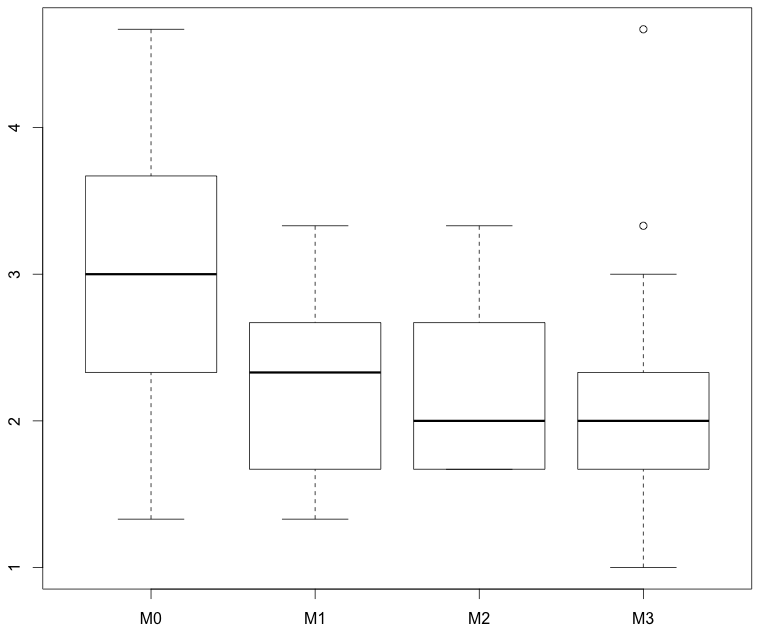
\includegraphics[width=0.3\linewidth]{img/studyload_fig8a}
		\label{fig:sload_8a}
	}
	\subfloat[Time planning]{
		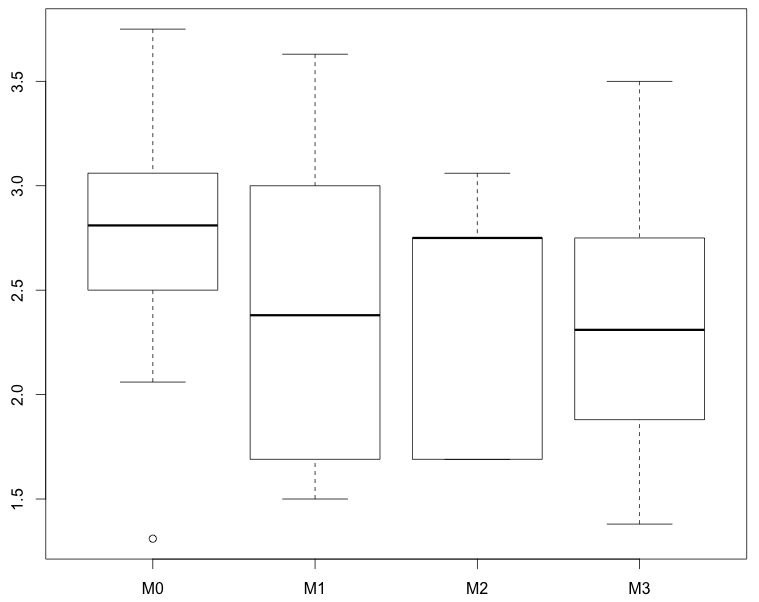
\includegraphics[width=0.3\linewidth]{img/studyload_fig8b}
		\label{fig:sload_8b}
	}	

      \caption{Boxplot with mean scores for significant subscales. 5) Strongly disagree; 4) Disagree; 3) Neutral; 2) Agree; 1) Strongly agree;}
      \label{fig:sload_8}
\end{figure}
\end{center}

\subsection{Impact of the timing in the notifications in self-regulation}

\begin{center}
\begin{figure}[ht]
\centering
	\subfloat[Contrast 1. Notifications pushed at fixed time of the day]{
		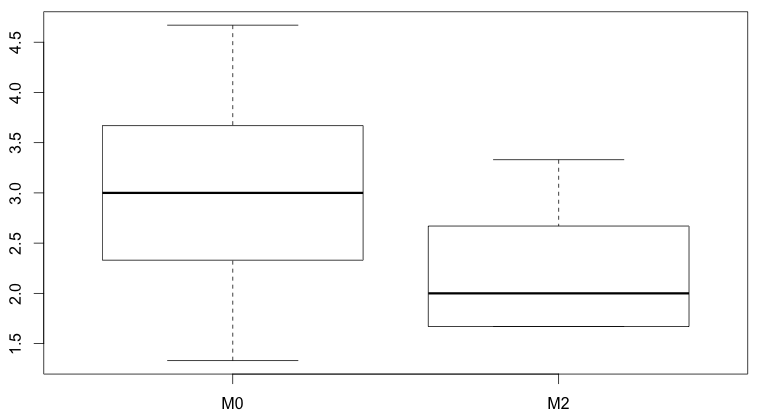
\includegraphics[width=0.3\linewidth]{img/studyload_fig9a}
		\label{fig:sload_9a}
	}
	\subfloat[Contrast 2. Notifications pushed on random basis in the time of the day]{
		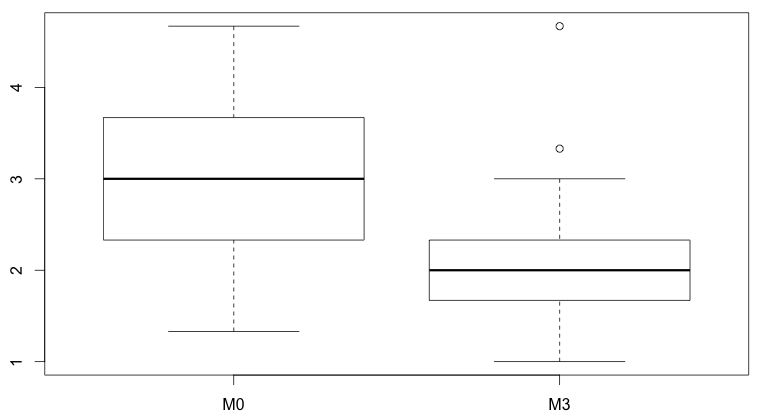
\includegraphics[width=0.3\linewidth]{img/studyload_fig9b}
		\label{fig:sload_9b}
	}	
      \caption{Boxplots with measure of means in �time management� subscale. 5) Strongly disagree; 4) Disagree; 3) Neutral; 2) Agree; 1) Strongly agree;}
      \label{fig:sload_9}
\end{figure}
\end{center}

\subsubsection{Patterns sampling study time}

\begin{figure}
     \centering
     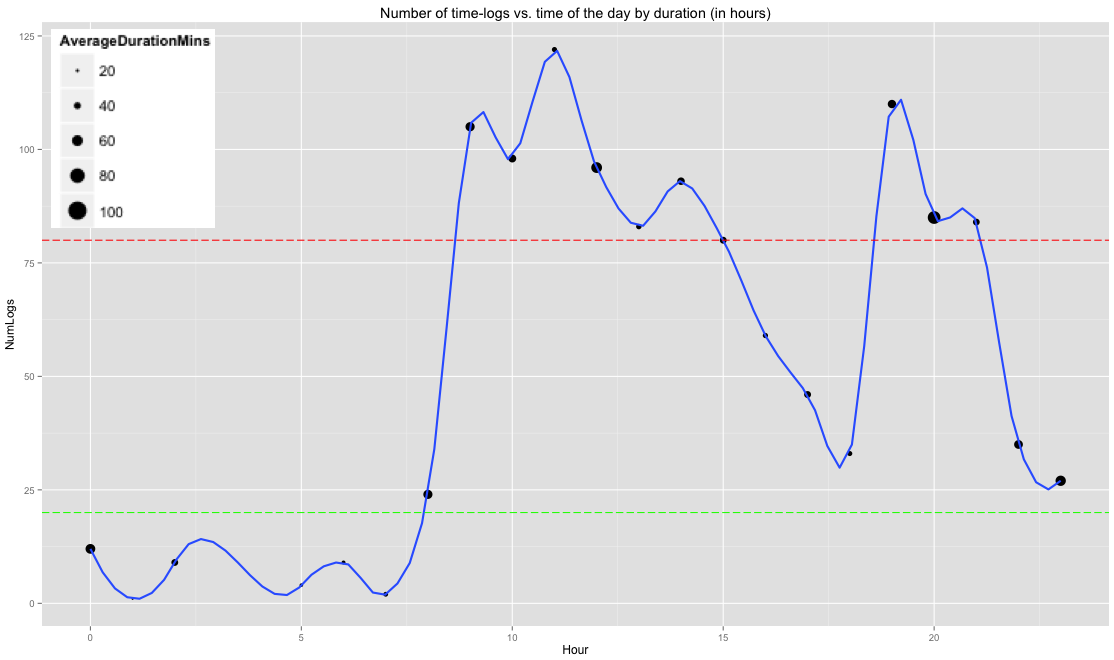
\includegraphics[width=0.7\linewidth]{img/studyload_fig10}
     \caption{Distribution of time logs along the day (n=1217). Y-axis represents the number of time-logs during the day. X-axis represents the time of the day. The width of the plot represents the mean duration of the time-logs for an hour.}
     \label{fig:sload_10}
\end{figure}


\begin{figure}
     \centering
     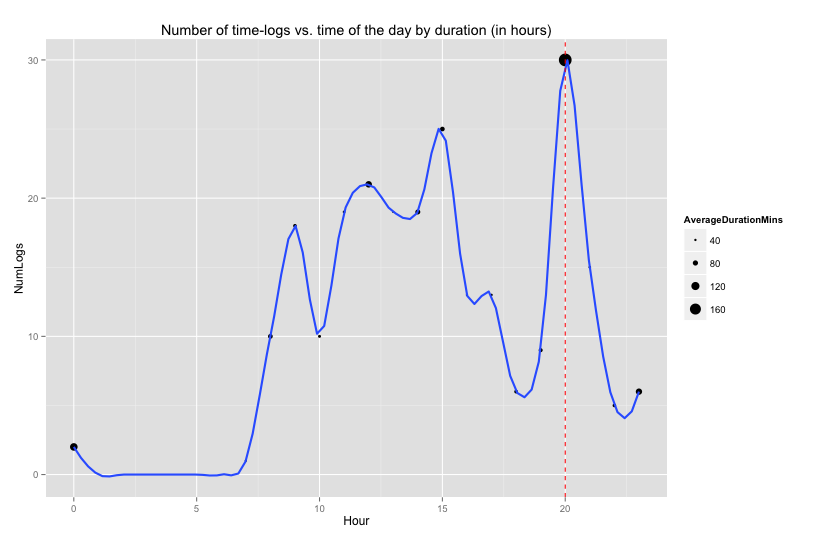
\includegraphics[width=0.7\linewidth]{img/studyload_fig11}
     \caption{Y-axis is the number of logs. X-axis is the time of the day. Relationship between the SMS notifications and students� time-log reactions. Submitting message in the evening at 20h. The thickness of the plot is the duration of the time-logs recorded}
     \label{fig:sload_11}
\end{figure}



\begin{figure}
     \centering
     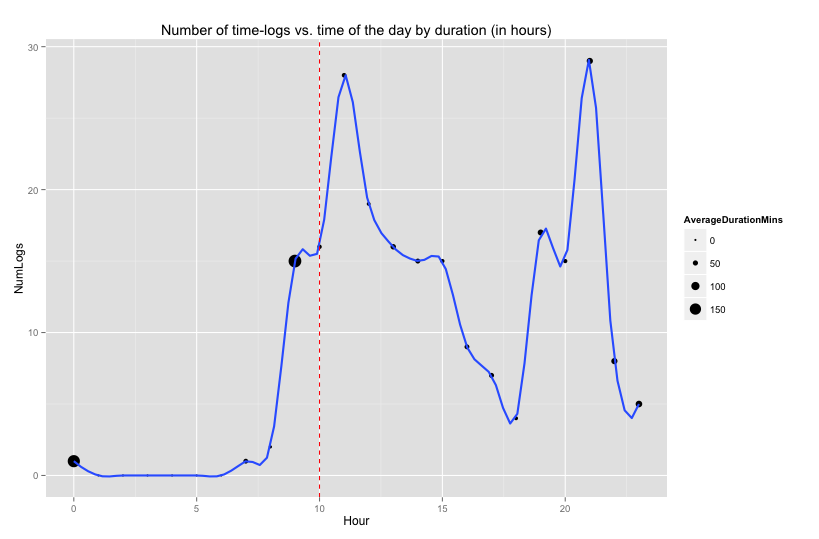
\includegraphics[width=0.7\linewidth]{img/studyload_fig12}
     \caption{Y-axis is the number of logs. X-axis is the time of the day. Relationship between the SMS notifications and students� time-logs reaction. Submitting message in the morning at 10h. The thickness of the plot is the duration of the time-logs recorded.}
     \label{fig:sload_12}
\end{figure}


\begin{figure}
     \centering
     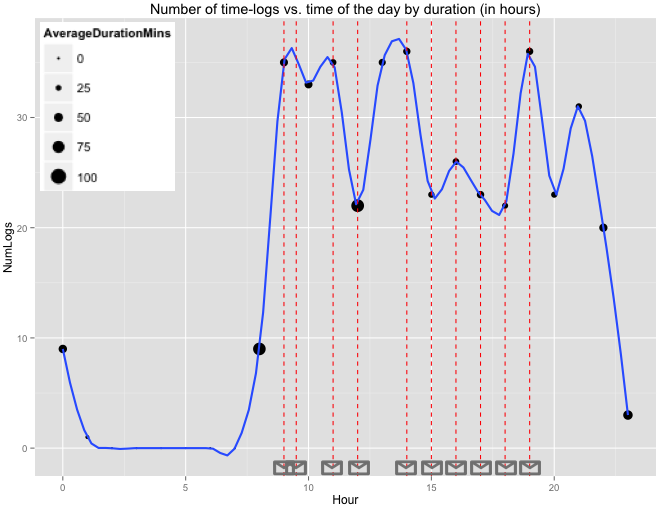
\includegraphics[width=0.7\linewidth]{img/studyload_fig13}
     \caption{Y-axis is the number of logs. X-axis is the time of the day. Relationship between the SMS notifications and students� time-logs reaction. Submitting message on random basis. The thickness of the plot is the duration of the time-logs recorded.}
     \label{fig:sload_13}
\end{figure}






\begin{table}[h]
  \centering
  \small
  \caption{Distribution of time-logs along the week}
  \label{tbl:studyload_table5}
  
\begin{tabular}{rrrc}
\hline
\textbf{Week day} & \textbf{Time-logs(n)} & \textbf{Minutes-logged(n)} & \textbf{\begin{tabular}[c]{@{}c@{}}Mean duration of\\ time-logs in minutes\end{tabular}} \\
\hline
Monday            & 12.00\% (n=146)       & 10.56\% (n=8499)           & 58.21                                                                                    \\
Tuesday           & 12.16\% (n=148)       & 15.39\% (n=12387)          & 83.69                                                                                    \\
Wednesday         & 12.90\% (n=157)       & 14.80\% (n=11913)          & 75.87                                                                                    \\
Thursday          & 20.95\% (n=255)       & 18.56\% (n=14937)          & 58.57                                                                                    \\
Friday            & 11.34\% (n=138)       & 10.69\% (n=8603)           & 62.34                                                                                    \\
Saturday          & 12.08\% (n=147)       & 11.75\% (n=9457)           & 64.33                                                                                    \\
Sunday            & 18.57\% (n=226)       & 18.25\% (n=14692)          & 65.00                                                                                   \\
\hline
\end{tabular}
\end{table}


\begin{table}[h]
  \centering
  \small
  \caption{Preferred timing. 5-Likert scale: 5.Most preferred; 3.Neutral; 1.Least preferred}
  \label{tbl:studyload_table6}
\begin{tabular}{ccc}
\hline
\textbf{10h M(SD)} & \textbf{20h M(SD)} & \textbf{Random M(SD)} \\ \hline
3.77(.83)          & 2.92(1.04)         & 2.85(.52)             \\ \hline
\end{tabular}
\end{table}



\subsubsection{How do students log their time}

\subsubsection{Correlation between time-logs and performance}


\subsection{Impact from the content of the notifications in self-regulation}



\begin{table}[h]
  \centering
  \small
  \caption{Planned contrast for time management and time planning subscales. * Significance: p < .05}
  \label{tbl:studyload_table7}
  
\begin{tabular}{rcccc}
\thickhline
\multicolumn{1}{c}{\textbf{\begin{tabular}[c]{@{}c@{}}Planned\\ contrast\end{tabular}}} & \multicolumn{2}{c}{\textbf{Contrast 1}} & \multicolumn{2}{c}{\textbf{Contrast 2}} \\ \thickhline
Measure                                                                                & TM                  & TP                & TM                  & TP                \\ \hline
M0                                                                                      & X                   & X                 & -                   & -                 \\ \hline
M1                                                                                      & (t=-2.14, p=.04)*   & (t=-1.19, p=.24)  & X                   & X                 \\ \hline
M2                                                                                      & -                   & -                 & (t=-2.52, p=.01)*   & (t=-.47, p=.15)   \\ \thickhline
\end{tabular}
\end{table}


\begin{center}
\begin{figure}[ht]
\centering
	\subfloat[Contrast 1. Notifications containing generic tips]{
		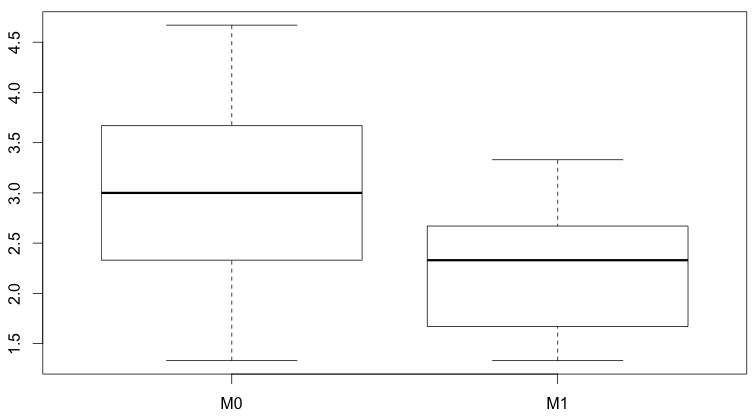
\includegraphics[width=0.3\linewidth]{img/studyload_fig14a}
		\label{fig:sload_14a}
	}
	\subfloat[Contrast 2. Notifications containing learning analytics]{
		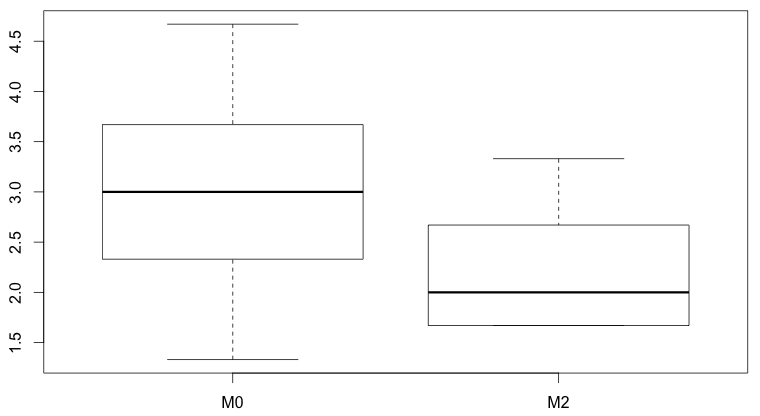
\includegraphics[width=0.3\linewidth]{img/studyload_fig14b}
		\label{fig:sload_14b}
	}		
      \caption{Boxplots with measure of means in �time management� subscale. 5) Strongly disagree; 4) Disagree; 3) Neutral; 2) Agree; 1) Strongly agree;}
      \label{fig:sload_14}
\end{figure}
\end{center}

\subsubsection{Preference in content and channels}




\begin{table}[h]
  \centering
  \small
  \caption{Preferred content. 5-Likert scale: 5.Most preferred; 3.Neutral; 1.Least preferred}
  \label{tbl:studyload_table8}
  
\begin{tabular}{cc}
\hline
\textbf{Learning analytics M(SD)} & \textbf{Tips M(SD)} \\ \hline
2.85(.69)                         & 2.92(1.04)          \\ \hline
\end{tabular}
\end{table}



\begin{table}[h]
  \centering
  \small
  \caption{Preferred channel. 5-Likert scale: 5.Most preferred; 3.Neutral; 1.Least preferred}
  \label{tbl:studyload_table9}


\begin{tabular}{cc}
\hline
\textbf{SMS notifications M(SD)} & \textbf{Chart visualizations M(SD)} \\ \hline
3.31(.95)                        & 3.46(1.13)                          \\ \hline
\end{tabular}
\end{table}





\begin{table}[h]
  \centering
  \small
  \caption{Perceived usefulness in Learning Analytics. 5-Likert scale. 5.Most useful; 3.Neutral; 1. Least useful}
  \label{tbl:studyload_table10}
  
\begin{tabular}{ccc}
\hline
\textbf{Personal M(SD)} & \textbf{Social M(SD)} & \textbf{Teacher M(SD)} \\ \hline
3.69(.85)               & 3.46(.88)             & 3.38(.96)              \\ \hline
\end{tabular}
\end{table}



\subsection{Usability of the tool}





\begin{table}[h]
  \centering
  \footnotesize
  \caption{Summary of interactions to accomplish a time-log. (* Number of actions / Number of clicks)}
  \label{tbl:studyload_table11}
  


\begin{tabular}{|c|c|c|c|}
\hline
\multicolumn{2}{|c|}{\textbf{LearnTracker for Android}}                                                                                                            & \multicolumn{2}{c|}{\textbf{Multiplatform web interface}}                                                                                                                           \\
\hline
\textbf{Minimum}                                                      & \textbf{Maximum}                                                                           & \textbf{Minimum}                                                                        & \textbf{Maximum}                                                                           \\
                                                                      & \begin{tabular}[c]{@{}c@{}}1 click to \\ start app\end{tabular}                            & \begin{tabular}[c]{@{}c@{}}1 click URL\\ on SMS\end{tabular}                            & \begin{tabular}[c]{@{}c@{}}1 click URL\\ on SMS\end{tabular}                               \\
\begin{tabular}[c]{@{}c@{}}1 click select\\ 1st activity\end{tabular} & \begin{tabular}[c]{@{}c@{}}2 clicks to scroll \\ and select\\ bottom activity\end{tabular} & \begin{tabular}[c]{@{}c@{}}1 click to display \\ HH scroll\\ 1st activity\end{tabular}  & \begin{tabular}[c]{@{}c@{}}2 clicks to scroll \\ and select\\ bottom activity\end{tabular} \\
\begin{tabular}[c]{@{}c@{}}1 click to \\ check-in\end{tabular}        & \begin{tabular}[c]{@{}c@{}}2 scroll bottom \\ HH\end{tabular}                              & \begin{tabular}[c]{@{}c@{}}1 clicks to \\ select HH\end{tabular}                        & \begin{tabular}[c]{@{}c@{}}1 click to \\ display HH scroll\end{tabular}                    \\
\begin{tabular}[c]{@{}c@{}}1 click to \\ check-out\end{tabular}       & \begin{tabular}[c]{@{}c@{}}2 scroll bottom\\ MM\end{tabular}                               & \begin{tabular}[c]{@{}c@{}}1 click on\\ �done�\end{tabular}                             & \begin{tabular}[c]{@{}c@{}}2 clicks to \\ scroll and select\\ bottom HH\end{tabular}       \\
                                                                      & \begin{tabular}[c]{@{}c@{}}1 click fast-fwd \\ asynch. log\end{tabular}                    & \begin{tabular}[c]{@{}c@{}}1 click to display \\ MM scroll \\ 1st activity\end{tabular} & 1 click on �done�                                                                          \\
                                                                      &                                                                                            & \begin{tabular}[c]{@{}c@{}}1 clicks to\\ select MM\end{tabular}                         & \begin{tabular}[c]{@{}c@{}}1 click to display \\ MM scroll\end{tabular}                    \\
                                                                      &                                                                                            & 1 click on �done�                                                                       & \begin{tabular}[c]{@{}c@{}}2 clicks to scroll \\ and select\\ bottom MM\end{tabular}       \\
                                                                      &                                                                                            & 1 click on �send�                                                                       & 1 click on �done�                                                                          \\
                                                                      &                                                                                            &                                                                                         & 1 click on �send�                                                                          \\
\hline                                                                      
\textbf{4/4}                                                          & \textbf{5/8}                                                                               & \textbf{8/8}                                                                            & \textbf{9/12}                                                                             \\
\hline
\end{tabular}
  



\end{table}



\section{Discussion}


\subsection{Interpretation of the results}

\subsection{Limitations}


\subsection{Significance of the study}

